%%%%%%%%%%%%%%%%%%%%%%%%%%%%%%%%%%%%%%%%%%%%%%%%%%%%
% Document type, global settings, and packages
%%%%%%%%%%%%%%%%%%%%%%%%%%%%%%%%%%%%%%%%%%%%%%%%%%%%

\documentclass[12pt]{report}   %12 point font for Times New Roman
\usepackage[a4paper, left=1.5in, right=1in, top=1in, bottom=1in]{geometry}
\usepackage{setspace}  %use this package to set linespacing as desired
\usepackage[english]{babel}
\usepackage{times}  %set Times New Roman as the font
\usepackage[utf8]{inputenc}
\usepackage{microtype}
\usepackage{graphicx}  %for images and plots
\usepackage[explicit]{titlesec}  %title control and formatting
\usepackage[titles]{tocloft}  %table of contents control and formatting
\usepackage{ulem}  %for underlined section titles
\usepackage[backend=bibtex, sorting=nty, bibstyle=nature, date=year, intitle=true, doi=false, isbn=false, url=false, clearlang=true]{biblatex}
\usepackage{yfonts}
\DeclareTextFontCommand{\textgoth}{\gothfamily}
%reference manager
\usepackage[bookmarks=true, hidelinks]{hyperref}
\usepackage[page]{appendix}  %for appendices
\usepackage{rotating}  %for rotated, landscape images
\usepackage{amsmath}
\usepackage{mathtools}
\usepackage[rightcaption]{sidecap}
\usepackage{csquotes}
\usepackage{wrapfig}
\usepackage{afterpage}
\usepackage{fancyhdr}
\usepackage{adjustbox}
\usepackage{listings}
\usepackage{subcaption}

\usepackage{pdfpages}
\newcommand\blankpage{
    \null
    \thispagestyle{empty}
    \addtocounter{page}{-1}
    \newpage
    }

%%%%%%%%%%%%%%%%%%%%%%%%%%%%%%%%%%%
% Bibliography
%%%%%%%%%%%%%%%%%%%%%%%%%%%%%%%%%%%

%Add your bibliography file here
\addbibresource{References.bib}

% prevent certain fields in references from printing in bibliography

\AtEveryBibitem{\clearfield{note}}
\AtEveryBibitem{\clearlist{note}}

\renewbibmacro*{title}{%
  \ifboolexpr{
    test {\iffieldundef{title}}
    and
    test {\iffieldundef{subtitle}}
  }
    {}
    {\printtext{%
     \printtext[titlecase]{\usefield{\uline}{title}}%
     \setunit{\subtitlepunct}%
     \printfield[titlecase]{subtitle}}%
     \newunit}%
  \printfield{titleaddon}}

\renewbibmacro*{booktitle}{%
  \ifboolexpr{
    test {\iffieldundef{booktitle}}
    and
    test {\iffieldundef{booksubtitle}}
  }
    {}
    {\printtext{%
     \printtext[titlecase]{\usefield{\uline}{booktitle}}%
     \setunit{\subtitlepunct}%
     \printfield[titlecase]{booksubtitle}}%
     \newunit}%
  \printfield{booktitleaddon}}

\renewbibmacro*{journal}{%
  \ifboolexpr{
    test {\iffieldundef{journaltitle}}
    and
    test {\iffieldundef{journalsubtitle}}
  }
    {}
    {\printtext[journaltitle]{%
       \printfield[titlecase]{\usefield{\uline}{journaltitle}}%
       \setunit{\subtitlepunct}%
       \printfield[titlecase]{journalsubtitle}}}}
%%%%%%%%%%%%%%%%%%%%%%
% Start of Document
%%%%%%%%%%%%%%%%%%%%%%

\begin{document}
\doublespacing  %set line spacing

%%%%%%%%%%%%%%%%%%%%%%%%%%%%%%%%%%%%%
% Title Page
%%%%%%%%%%%%%%%%%%%%%%%%%%%%%%%%%%%%%


\includepdf{TitlePage.pdf}
\currentpdfbookmark{Title Page}{titlePage}  %add PDF bookmark for this page

\includepdf[]{ApprovalSheet.pdf}

\includepdf[pages = 1-2]{DecandCert.pdf}

%%%%%%%%%%%%%%%%%%%%%%%%%%%%%%%%%%%%%
% Approval Page
%%%%%%%%%%%%%%%%%%%%%%%%%%%%%%%%%%%%%

%
\includepdf{ApprovalPage/ApprovalPage.pdf}

%%%%%%%%%%%%%%%%%%%%%%%%%%%%%%%%%%%%%
% Declaration
%%%%%%%%%%%%%%%%%%%%%%%%%%%%%%%%%%%%%

%
\includepdf{Declaration/Declaration.pdf}

%%%%%%%%%%%%%%%%%%%%%%%%%%%%%%%%%%%%%
% Certificate
%%%%%%%%%%%%%%%%%%%%%%%%%%%%%%%%%%%%%

%
\includepdf{Certificate/Certificate.pdf}

%%%%%%%%%%%%%%%%%%%%%%%%%%%%%%%%%%%%%
% Acknowledgments
%%%%%%%%%%%%%%%%%%%%%%%%%%%%%%%%%%%%%

\pagenumbering{roman}
\addcontentsline{toc}{chapter}{Acknowledgments}
\setcounter{page}{1} % set the page number appropriately based on the number of intro pages
\clearpage
\begin{centering}
{\Large \textbf{ACKNOWLEDGEMENTS}}\\
\vspace{\baselineskip}
\end{centering}

%Insert your dedication text here
First and Foremost, I praise Almighty God for giving me this beautiful life full of oppurtunities and for always being there with me in my times of joys and sorrow.

I would like to express my deep and sincere thanks to \textbf{Dr. Twinkle R. Singh} for her continuous support of my project work. She motivated me, provided valuable guidance and gave stimulating suggestions which were instrumental in successful completion of my project work and writing of this dissertation.

It gives me immense pleasure to record the love and affection towards my family, especially to my parents for their blessings, inspiration and well wishes in my life. I would like to thank my brother for his support and help through every phase of my life.

I have always been fortunate to be in the company of wonderful and caring friends,who have been a great source of joy for me, specially \textbf{Aniruddha Deshmukh, Sumeet Kumar, Soumit Jana} and \textbf{Abhishek Kumar} for their companionship during difficult times.
\vspace{4em}
\begin{flushright}

Rohit Mittel \\
Surat.
\end{flushright}
\clearpage
%\pagenumbering{gobble}  %remove page number on summary page


\addtocontents{toc}{\cftpagenumbersoff{chapter}} 

\currentpdfbookmark{Acknowledgments}{acknowledgments}
\addtocontents{toc}{\cftpagenumberson{chapter}} 

%%%%%%%%%%%%%%%%%%%%%%%%%%%%%%%%%%%%%
% Preface
%%%%%%%%%%%%%%%%%%%%%%%%%%%%%%%%%%%%%
\addcontentsline{toc}{chapter}{Preface}
\input{Chapters/Preface.tex}


\addtocontents{toc}{\cftpagenumbersoff{chapter}} 

\currentpdfbookmark{Preface}{preface}
\addtocontents{toc}{\cftpagenumberson{chapter}}
%%%%%%%%%%%%%%%%%%%%%%%%%%%%%%%%%%%%%
% Table of Contents
%%%%%%%%%%%%%%%%%%%%%%%%%%%%%%%%%%%%%

%Format for Table of Contents
\renewcommand{\cftchapdotsep}{\cftdotsep}  %add dot separators
\renewcommand{\cftchapfont}{\bfseries}  %set title font weight
\renewcommand{\cftchappagefont}{}  %set page number font weight
\renewcommand{\cftchappresnum}{Chapter }
\renewcommand{\cftchapaftersnum}{:}
\renewcommand{\cftchapnumwidth}{5em}
\renewcommand{\cftchapafterpnum}{\vskip\baselineskip} %set correct spacing for entries in single space environment
\renewcommand{\cftsecafterpnum}{\vskip\baselineskip}  %set correct spacing for entries in single space environment
\renewcommand{\cftsubsecafterpnum}{\vskip\baselineskip} %set correct spacing for entries in single space environment
\renewcommand{\cftsubsubsecafterpnum}{\vskip\baselineskip}  %set correct spacing for entries in single space environment

%format title font size and position (this also applys to list of figures and list of tables)
\titleformat{\chapter}[display]
{\normalfont\bfseries\filcenter}{\chaptertitlename\ \thechapter}{0pt}{\MakeUppercase{#1}}

\renewcommand\contentsname{{\Large Table of Contents}}

\begin{singlespace}
\tableofcontents
\end{singlespace}

\currentpdfbookmark{Table of Contents}{TOC}

\clearpage

%%%%%%%%%%%%%%%%%%%%%%%%%%%%%%%%%%%%%
% List of figures and tables
%%%%%%%%%%%%%%%%%%%%%%%%%%%%%%%%%%%%%

\addcontentsline{toc}{chapter}{List of Tables}
\begin{singlespace}
	\setlength\cftbeforetabskip{\baselineskip}  %manually set spacing between entries
	\listoftables
\end{singlespace}

\clearpage

\addcontentsline{toc}{chapter}{List of Figures}
\begin{singlespace}
\setlength\cftbeforefigskip{\baselineskip}  %manually set spacing between entries
\listoffigures
\end{singlespace}

\clearpage

%%%%%%%%%%%%%%%%%%%%%%%%%%%%%%%%%%%%%%%%%%%%%%%%%%%%%%%%%%%%%%%%%
% This is the Summary (abstract should be separate document)
%%%%%%%%%%%%%%%%%%%%%%%%%%%%%%%%%%%%%%%%%%%%%%%%%%%%%%%%%%%%%%%%%

%\input{summary.tex}

%%%%%%%%%%%%%%%%%%%%%%%%%%%%
%
% Chapters
%
%%%%%%%%%%%%%%%%%%%%%%%%%%%%

%%%%%%%%%%%%%%%%%%%%%%
% formatting
%%%%%%%%%%%%%%%%%%%%%%

% resume page numbering for rest of document
\clearpage
\pagenumbering{arabic}
\setcounter{page}{1} % set the page number appropriately

% Adjust chapter title formatting
\titleformat{\chapter}[display]
{\normalfont\bfseries\filcenter}{\MakeUppercase\chaptertitlename\ \thechapter}{0pt}{\MakeUppercase{#1}}  %spacing between titles
\titlespacing*{\chapter}
  {0pt}{0pt}{30pt}	%controls vertical margins on title
  
% Adjust section title formatting
\titleformat{\section}{\normalfont\bfseries}{\thesection}{1em}{#1}

% Adjust subsection title formatting
\titleformat{\subsection}{\normalfont}{\uline{\thesubsection}}{0em}{\uline{\hspace{1em}#1}}

% Adjust subsubsection title formatting
\titleformat{\subsubsection}{\normalfont\itshape}{\thesubsubsection}{1em}{#1}

%%%%%%%%%%%%%%%%
% Chapter 1
%%%%%%%%%%%%%%%%

\input{Chapters/Chapter1.tex}
\afterpage{\blankpage}

%%%%%%%%%%%%%%%%
% Chapter 2
%%%%%%%%%%%%%%%%

\input{Chapters/Chapter2.tex}
\afterpage{\blankpage}

%%%%%%%%%%%%%%%%
% Chapter 3
%%%%%%%%%%%%%%%%

\input{Chapters/Chapter3.tex}
\afterpage{\blankpage}

%%%%%%%%%%%%%%%%
% Chapter 4
%%%%%%%%%%%%%%%%

\input{Chapters/Chapter4.tex}
\afterpage{\blankpage}

%%%%%%%%%%%%%%%%
% Chapter 5
%%%%%%%%%%%%%%%%

\input{Chapters/Chapter5.tex}
\afterpage{\blankpage}

%%%%%%%%%%%%%%%%
% Chapter 6
%%%%%%%%%%%%%%%%

\input{Chapters/Chapter6.tex}
\afterpage{\blankpage}


%%%%%%%%%%%%%%%%
% Appendices
%%%%%%%%%%%%%%%%

%\input{appendix.tex}

%%%%%%%%%%%%%%%%
% References
%%%%%%%%%%%%%%%%

\begin{singlespace}  % use single-line spacing for multi-line text within a single reference
    \microtypesetup{protrusion=false}
	\setlength\bibitemsep{\baselineskip}  %manually set separation between items in bibliography to double space
    \nocite{*}
	\printbibliography[title={\LARGE References}]
\end{singlespace}

\addcontentsline{toc}{chapter}{References}  %add References section to Table of Contents

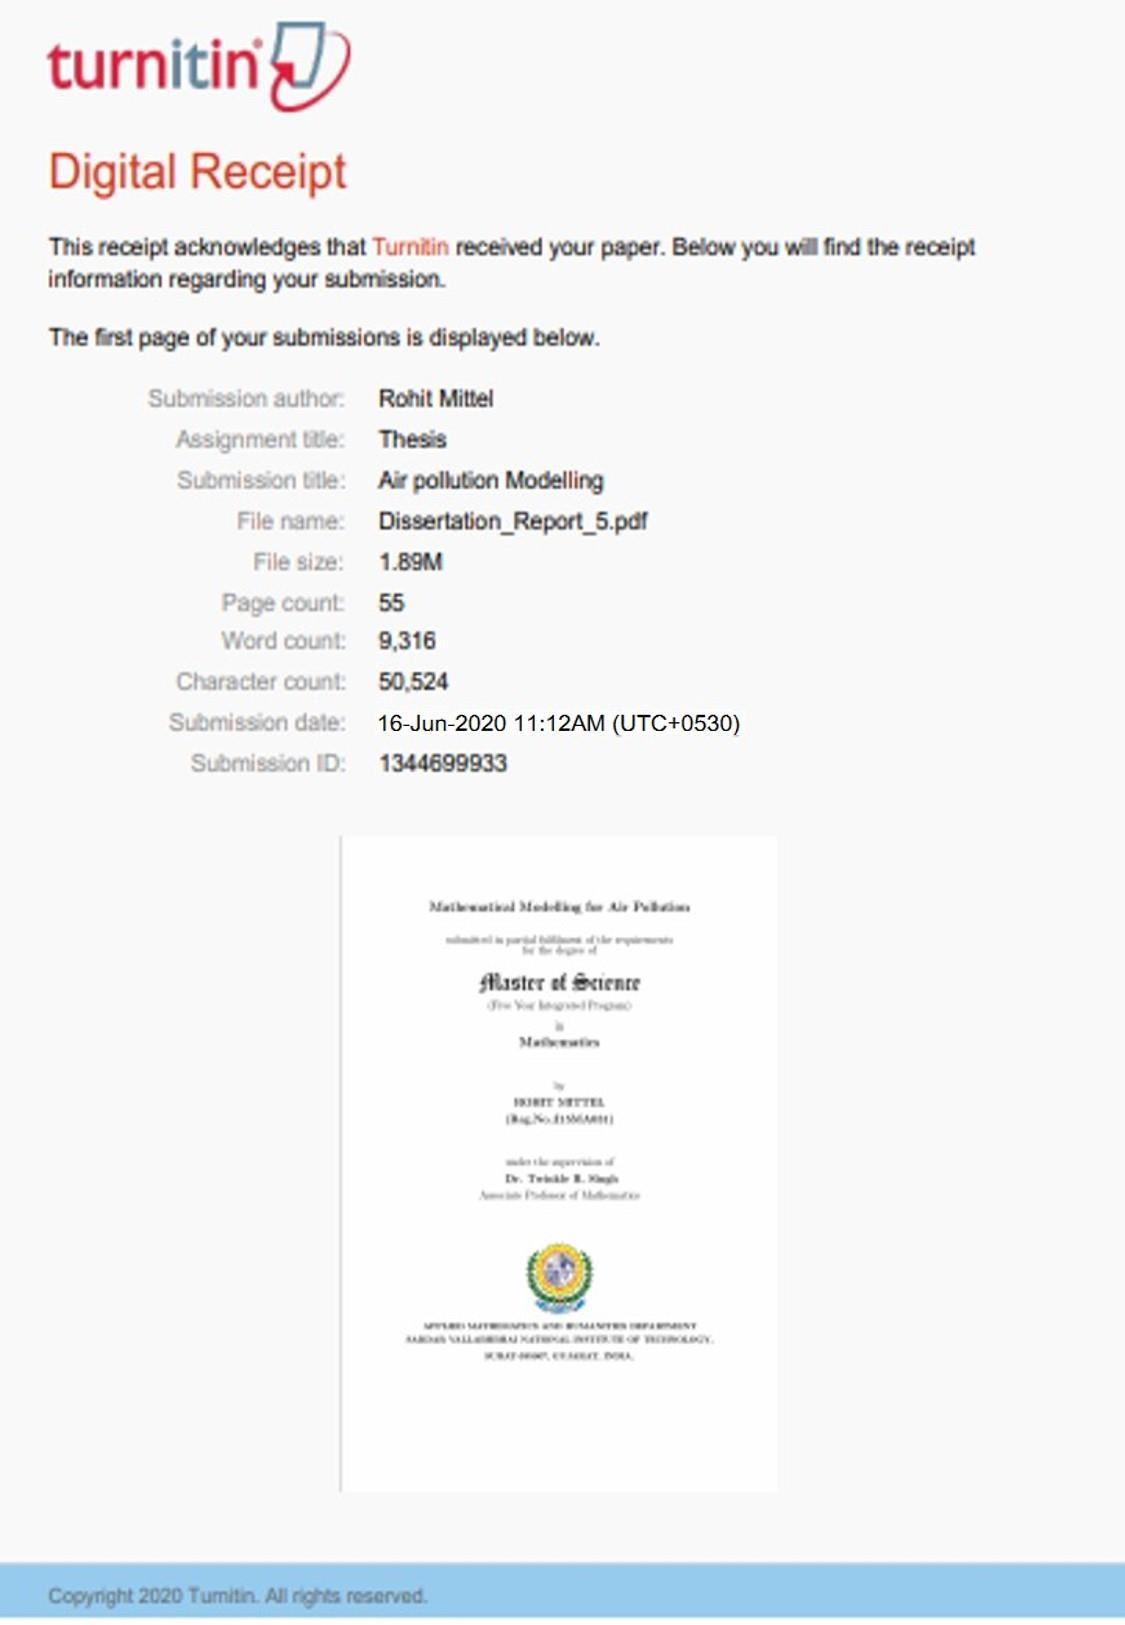
\includepdf{ReportReceipt.pdf}

\includepdf[pages = 1-3]{Plagiarism Report.pdf}

\end{document}